\chapter[past]{Overview of Past Activities}
 [
  This chapter is the showcase one: it demonstrates the figures, tables, equations, boxes and cross-references provided by the template. \\
  All the text is placeholder text, so do not look for any meaning in it. Replace it with a summary of your own activities.
 ]

\section[past_topic]{A First Research Topic}

\subsection[past_topic_context]{Context}

Lorem ipsum dolor sit amet, consectetur adipiscing elit~\cite{ipsum1998foundational}.
Sed do eiusmod tempor incididunt ut labore et dolore magna aliqua, as later formalized in \cite{tempor2009textbook} and revisited by \cite{amet2017seminal}.
My own contributions on this topic are \cite{lastname2015thesis}, \cite{lastname2021journal} and \cite{lastname2022conference}.

\begin{boxenv}[past_definition]{Definition}[Placeholder object]
    A \emph{placeholder object} is any object that carries no meaning, and only exists to occupy the space where a real one will eventually be written.
    Note that the counter of this box is independent from the one of \nameref{introduction_challenge}, since the types differ.
\end{boxenv}

Placeholder objects satisfy the property stated in \nameref{past_theorem}, whose proof is immediate.

\begin{boxenv}[past_theorem]{Theorem}[Conservation of placeholders]
    Let $\mathcal{P}$ be a set of placeholder objects, and $f$ a placeholder map.
    Then $f(\mathcal{P})$ is a set of placeholder objects.
\end{boxenv}

\begin{proof}{past_theorem}
    By definition, a placeholder object carries no meaning.
    Applying a placeholder map to a meaningless object cannot create meaning, hence the result.
\end{proof}

\subsection[past_topic_method]{Method}

The overall pipeline is sketched in \nameref{example_diagram}: a placeholder object, as introduced in \nameref{past_definition}, is fed to a placeholder model that produces a placeholder output.
The placeholder loss we minimize is given in \nameref{past_equation}, where $\bm{x}$ denotes an input, $\bm{y}$ its target, and $\theta$ the parameters of the model.

\begin{equation}[past_equation]
    \mathcal{L}(\theta) = \frac{1}{N} \sum_{i = 1}^{N} \left\| f_\theta(\bm{x}_i) - \bm{y}_i \right\|_2^2 + \lambda \left\| \theta \right\|_2^2
\end{equation}

Note that equations, figures and tables are numbered continuously across the whole document, and not per chapter.
This is on purpose: it makes cross-references such as \nameref{past_equation} unambiguous.

\paragraph[past_topic_runin]{Run-in headings} Below \texttt{\textbackslash subsubsection}, two run-in levels are available. This one is a \texttt{\textbackslash paragraph}: bold, in the colour of the titles, and referable like any other level through \nameref{past_topic_runin}.

\subparagraph{One level deeper} A \texttt{\textbackslash subparagraph} is the same run-in separator in the same colour, but in the normal font weight. Neither level is numbered, and neither appears in the table of contents.

\begin{figure}[example_diagram]{The pipeline used throughout this placeholder chapter. A figure is declared with \texttt{\textbackslash begin\{figure\}[label]\{caption\}}, and takes no placement specifier: the caption is the second, mandatory argument.}
    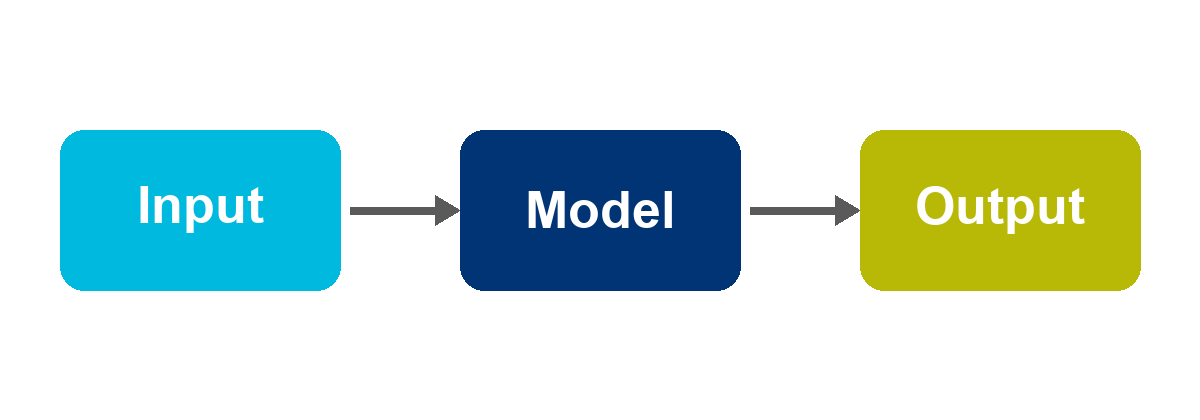
\includegraphics[width=0.9\linewidth]{manuscript/figures/example_diagram.png}
\end{figure}

\subsection[past_topic_results]{Results}

Results are reported in \nameref{example_figure}, and summarized in \nameref{example_table}.
As expected, the placeholder model in \nameref{example_figure}~\nameref{example_figure_curves} outperforms the placeholder baseline, which is exactly what a placeholder result is supposed to do.

\begin{figure}[example_figure]{A figure made of several subfigures. Subfigures take a label, a width, and a caption, and can be referred to individually, as in \nameref{example_figure_image}, or as a whole through \nameref{example_figure}.}
    \begin{subfigure}[example_figure_image]{0.48\linewidth}{A raster image, included with the usual \texttt{\textbackslash includegraphics}.}
        
\includegraphics[width=\linewidth]{manuscript/figures/example_image.png}
    \end{subfigure}
    \hfill
    \begin{subfigure}[example_figure_curves]{0.48\linewidth}{A vector figure, generated by a script and included with \texttt{\textbackslash input}. \nameref{example_plot_model} The placeholder model; \nameref{example_plot_baseline} The placeholder baseline. Both markers are placed with \texttt{\textbackslash labeledText[label]\{text\}}, and recalled here with \texttt{\textbackslash nameref}.}
        % Example of a vector figure, meant to be included with \input{} inside a figure environment
% Such fragments are typically produced by a script, so that data and rendering stay in sync
% The tikzpicture environment is patched by the template to never overflow \linewidth

\begin{tikzpicture}

    \begin{axis}
        [
            height      = 5cm,
            width       = \linewidth,
            xlabel      = {Number of training epochs},
            ylabel      = {Placeholder metric},
            xmin        = 0, xmax = 20,
            ymin        = 0, ymax = 1,
            grid        = major,
            grid style  = {separatorColor},
            legend pos  = south east,
            legend cell align = left,
        ]

        \addplot[titlesColor, line width=1.5pt, mark=*, mark size=1.5pt] coordinates
            {
                (0, 0.10) (2, 0.38) (4, 0.55) (6, 0.66) (8, 0.73)
                (10, 0.78) (12, 0.82) (14, 0.84) (16, 0.86) (18, 0.87) (20, 0.87)
            };
        \addlegendentry{Placeholder model}

        \addplot[linksColor, line width=1.5pt, dashed, mark=square*, mark size=1.5pt] coordinates
            {
                (0, 0.10) (2, 0.30) (4, 0.44) (6, 0.53) (8, 0.59)
                (10, 0.63) (12, 0.66) (14, 0.68) (16, 0.69) (18, 0.70) (20, 0.70)
            };
        \addlegendentry{Placeholder baseline}

    \end{axis}

\end{tikzpicture}

    \end{subfigure}
\end{figure}

\begin{table}[example_table]{Placeholder results, on placeholder datasets. Tables follow the same convention as figures: \texttt{\textbackslash begin\{table\}[label]\{caption\}}.}
    \begin{tabular}{lcc}
        \hline
        \textbf{Dataset} & \textbf{Baseline} & \textbf{Placeholder model} \\
        \hline
        Placeholder-A    & $0.70 \pm 0.02$   & $\bm{0.87 \pm 0.01}$       \\
        Placeholder-B    & $0.61 \pm 0.03$   & $\bm{0.79 \pm 0.02}$       \\
        Placeholder-C    & $0.55 \pm 0.04$   & $\bm{0.68 \pm 0.03}$       \\
        \hline
    \end{tabular}
\end{table}

\section[past_collaborations]{Collaborations}

Beyond \nameref{past_topic}, I contributed to a few placeholder collaborations, listed below.
\acro{cnn_plural} were involved in most of them, which is a convenient excuse to demonstrate a variation: \verb|cnn_plural| carries no \verb|long| field and names \verb|cnn| in its \verb|alt| field, so the list of \nameref{glossary} holds no line of its own for it. Hovering it still shows \acroname{cnn_plural}, and clicking it leads to the \acro{cnn} entry.

\begin{boxenv*}{\faFlask~\cite{lastname2019chapter}}[\fullcite{lastname2019chapter}]
    A starred box, \texttt{boxenv*}, is not numbered.
    This makes it convenient to summarize a publication: the title of the box is the citation, and its subtitle the full reference.
    Lorem ipsum dolor sit amet, consectetur adipiscing elit, sed do eiusmod tempor incididunt.
\end{boxenv*}

\begin{boxenv*}{\faFlask~\cite{lastname2023workshop}}[\fullcite{lastname2023workshop}]
    Ut enim ad minim veniam, quis nostrud exercitation ullamco laboris nisi ut aliquip ex ea commodo consequat.
    Duis aute irure dolor in reprehenderit in voluptate velit esse cillum dolore eu fugiat nulla pariatur.
\end{boxenv*}

Online resources can be cited the same way, \eg \cite{placeholder_www}, and are gathered in their own section of the \nameref{bibliography}.
